\documentclass[11pt,a4paper]{article}
\usepackage[margin=2.2cm]{geometry}
\usepackage[T1]{fontenc}
\usepackage{lmodern}
\usepackage{amsmath,amssymb}
\usepackage{graphicx}
\usepackage{booktabs}
\usepackage{tabularx}
\usepackage{float}
\usepackage{enumitem}
\usepackage{xcolor}
\usepackage{tikz}
\usetikzlibrary{arrows.meta,positioning,calc}
\usepackage{caption}
\usepackage{subcaption}
\usepackage{hyperref}
\hypersetup{colorlinks=true, linkcolor=blue!60!black, urlcolor=blue!60!black}
\graphicspath{{../Question2/figures/}}

\title{AI651 -- Deep Learning for Space, Time and Graphs\\Assignment 2}
\author{Hafiz Muhammad Ahmad (25030011)\\[4pt]
\normalsize GitHub repository: \url{https://github.com/HMAhmadCS/DL4STG-PA2}}
\date{Fall 2026}

\begin{document}
\maketitle
\tableofcontents
\newpage

%======================================================================
\part*{Question 1 -- River Forecasting Proposal}
\addcontentsline{toc}{part}{Question 1 -- River Forecasting Proposal}
%======================================================================
%----------------------------------------------------------------------
\section{Architecture diagram}
%----------------------------------------------------------------------
\begin{figure}[H]
\centering
\resizebox{\textwidth}{!}{%
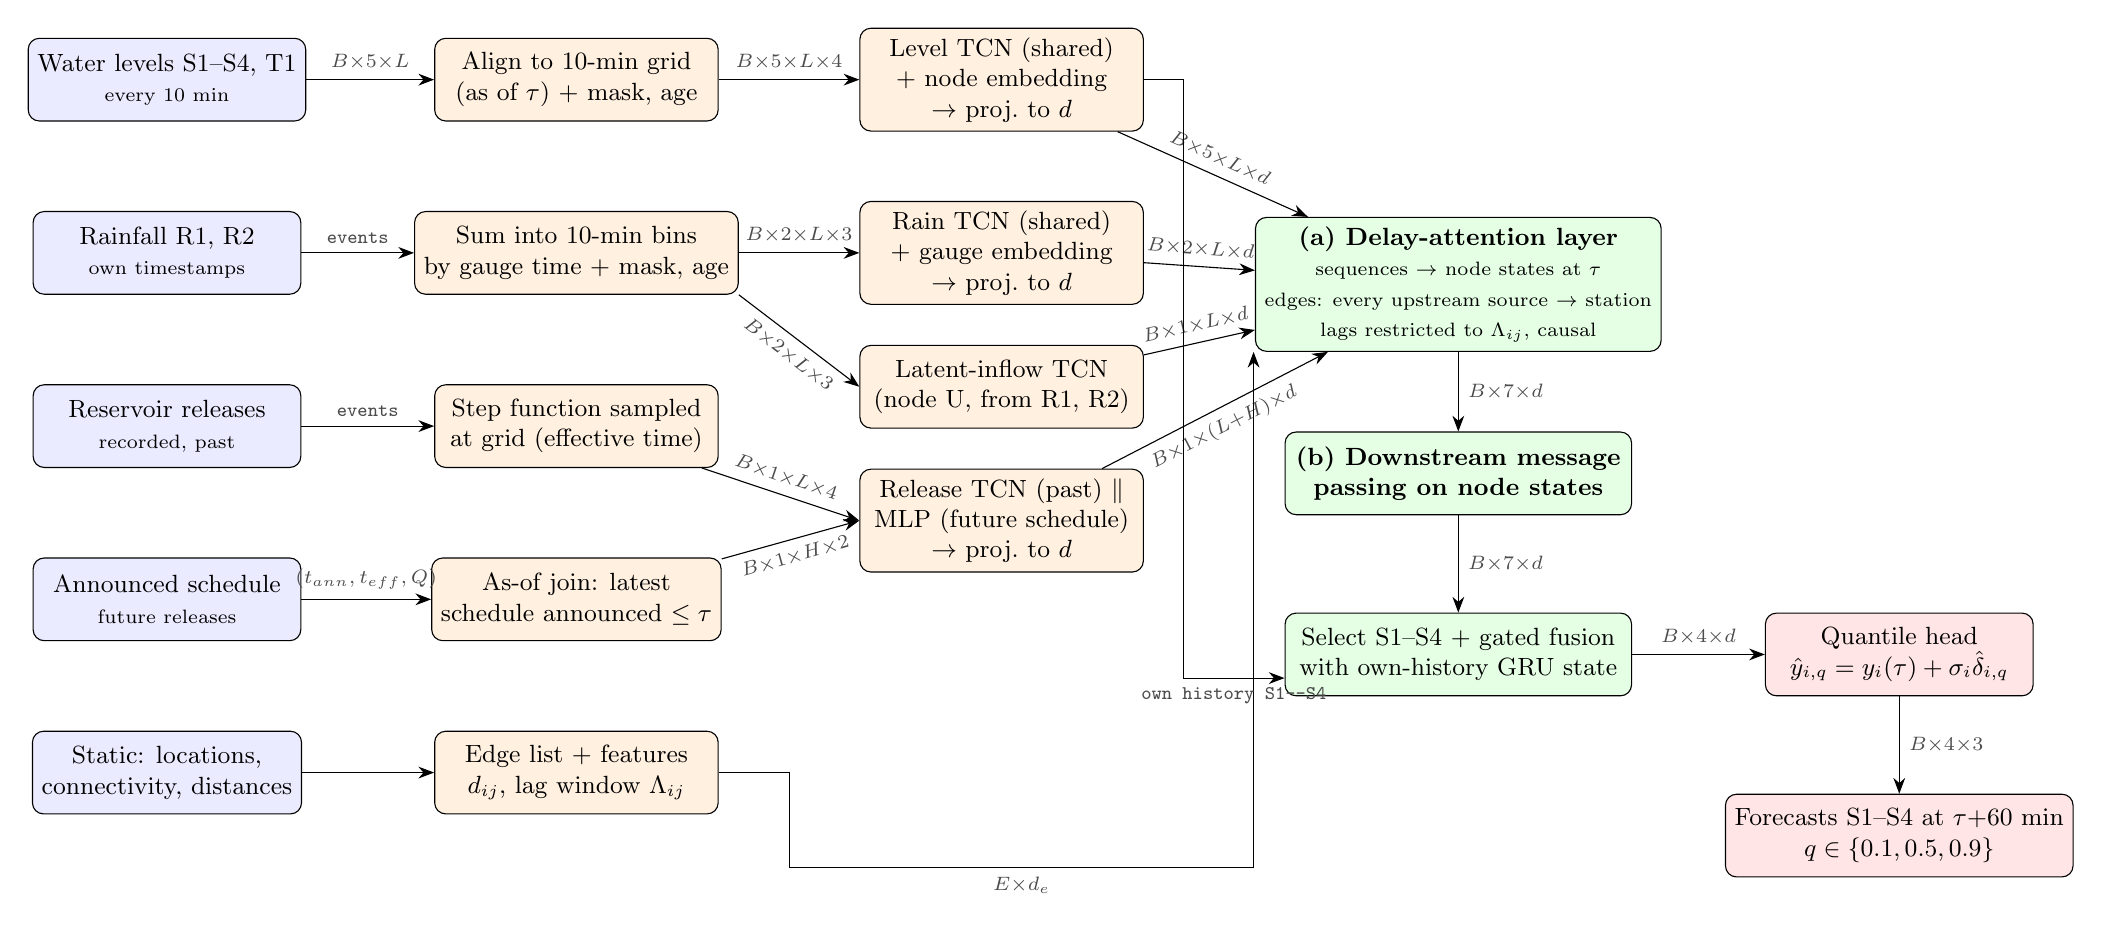
\begin{tikzpicture}[
  font=\small,
  src/.style={draw, rounded corners, fill=blue!8, align=center, minimum width=3.4cm, minimum height=1.05cm},
  blk/.style={draw, rounded corners, fill=orange!12, align=center, minimum width=3.6cm, minimum height=1.05cm},
  gnn/.style={draw, rounded corners, fill=green!10, align=center, minimum width=4.4cm, minimum height=1.05cm},
  outbox/.style={draw, rounded corners, fill=red!10, align=center, minimum width=3.4cm, minimum height=1.05cm},
  dim/.style={font=\scriptsize\ttfamily, text=black!70},
  >={Stealth[length=2mm]}]
% data sources
\node[src] (lev) at (0,0)     {Water levels S1--S4, T1\\\scriptsize every 10 min};
\node[src] (rain) at (0,-2.2) {Rainfall R1, R2\\\scriptsize own timestamps};
\node[src] (rel) at (0,-4.4)  {Reservoir releases\\\scriptsize recorded, past};
\node[src] (sch) at (0,-6.6)  {Announced schedule\\\scriptsize future releases};
\node[src] (sta) at (0,-8.8)  {Static: locations,\\connectivity, distances};
% alignment
\node[blk] (al1) at (5.2,0)     {Align to 10-min grid\\(as of $\tau$) + mask, age};
\node[blk] (al2) at (5.2,-2.2)  {Sum into 10-min bins\\by gauge time + mask, age};
\node[blk] (al3) at (5.2,-4.4)  {Step function sampled\\at grid (effective time)};
\node[blk] (al4) at (5.2,-6.6)  {As-of join: latest\\schedule announced $\le\tau$};
\node[blk] (al5) at (5.2,-8.8)  {Edge list + features\\$d_{ij}$, lag window $\Lambda_{ij}$};
% encoders (each ends with a linear projection to width d)
\node[blk] (enc1) at (10.6,0)    {Level TCN (shared)\\+ node embedding\\$\to$ proj.\ to $d$};
\node[blk] (enc2) at (10.6,-2.2) {Rain TCN (shared)\\+ gauge embedding\\$\to$ proj.\ to $d$};
\node[blk] (encu) at (10.6,-3.9) {Latent-inflow TCN\\(node U, from R1, R2)};
\node[blk] (enc3) at (10.6,-5.6) {Release TCN (past) $\Vert$\\MLP (future schedule)\\$\to$ proj.\ to $d$};
% graph
\node[gnn] (graph) at (16.4,-2.6) {\textbf{(a) Delay-attention layer}\\\scriptsize sequences $\to$ node states at $\tau$\\
  \scriptsize edges: every upstream source $\to$ station\\\scriptsize lags restricted to $\Lambda_{ij}$, causal};
\node[gnn] (mp) at (16.4,-5.0) {\textbf{(b) Downstream message}\\\textbf{passing on node states}};
\node[gnn] (fuse) at (16.4,-7.3) {Select S1--S4 + gated fusion\\with own-history GRU state};
% outputs
\node[outbox] (head) at (22.0,-7.3) {Quantile head\\$\hat y_{i,q}=y_i(\tau)+\sigma_i\hat\delta_{i,q}$};
\node[outbox] (fc) at (22.0,-9.6) {Forecasts S1--S4 at $\tau{+}60$ min\\$q\in\{0.1,0.5,0.9\}$};
% arrows
\draw[->] (lev) -- node[above, dim]{$B{\times}5{\times}L$} (al1);
\draw[->] (rain) -- node[above, dim]{events} (al2);
\draw[->] (rel) -- node[above, dim]{events} (al3);
\draw[->] (sch) -- node[above, dim]{$(t_{ann},t_{eff},Q)$} (al4);
\draw[->] (sta) -- (al5);
\draw[->] (al1) -- node[above, dim]{$B{\times}5{\times}L{\times}4$} (enc1);
\draw[->] (al2) -- node[above, dim]{$B{\times}2{\times}L{\times}3$} (enc2);
\draw[->] (al2.south east) -- node[below, dim, sloped]{$B{\times}2{\times}L{\times}3$} (encu.west);
\draw[->] (al3) -- node[above, dim, sloped]{$B{\times}1{\times}L{\times}4$} (enc3.west);
\draw[->] (al4) -- node[below, dim, sloped]{$B{\times}1{\times}H{\times}2$} (enc3.west);
\draw[->] (enc1) -- node[above, dim, sloped]{$B{\times}5{\times}L{\times}d$} (graph);
\draw[->] (enc2) -- node[above, dim, sloped]{$B{\times}2{\times}L{\times}d$} (graph);
\draw[->] (encu) -- node[above, dim, sloped]{$B{\times}1{\times}L{\times}d$} (graph);
\draw[->] (enc3) -- node[below, dim, sloped]{$B{\times}1{\times}(L{+}H){\times}d$} (graph);
\draw[->] (al5.east) -- ++(0.9,0) -- ++(0,-1.2) -| node[pos=0.25, below, dim]{$E{\times}d_e$} ([xshift=-2.6cm]graph.south);
\draw[->] (graph) -- node[right, dim]{$B{\times}7{\times}d$} (mp);
\draw[->] (mp) -- node[right, dim]{$B{\times}7{\times}d$} (fuse);
\draw[->] (enc1.east) -- ++(0.5,0) |- node[pos=0.75, below, dim]{own history S1--S4} ([yshift=-0.3cm]fuse.west);
\draw[->] (fuse) -- node[above, dim]{$B{\times}4{\times}d$} (head);
\draw[->] (head) -- node[right, dim]{$B{\times}4{\times}3$} (fc);
\end{tikzpicture}}
\caption{LADS-GNN. $B$: batch of issuance times $\tau$; $L=72$ history steps (12\,h at
$\Delta=10$\,min); $H=6$ future steps (1\,h); $d=64$ embedding width; $E$: number of directed edges.
\textbf{Alignment:} every source is put on the issuance-anchored grid
$\{\tau-71\Delta,\dots,\tau\}$ (and $\{\tau+\Delta,\dots,\tau+6\Delta\}$ for the announced schedule)
before encoding. \textbf{Projection:} each encoder ends in a linear layer to width $d$, so
sources with different raw features (4, 3, 4 and 2 channels) can be mixed in the graph.
\textbf{Reshaping:} the graph works on 7 nodes (Res, T1, U, S1--S4); the 4 station rows are
selected ($B{\times}7{\times}d\to B{\times}4{\times}d$) and the head outputs 3 quantiles per
station ($B{\times}4{\times}3$). The own-history GRU path (bottom) is taken from the level
encoder for S1--S4. The node graph is shown in Figure~\ref{fig:graph}.}
\label{fig:arch}
\end{figure}

\begin{figure}[H]
\centering
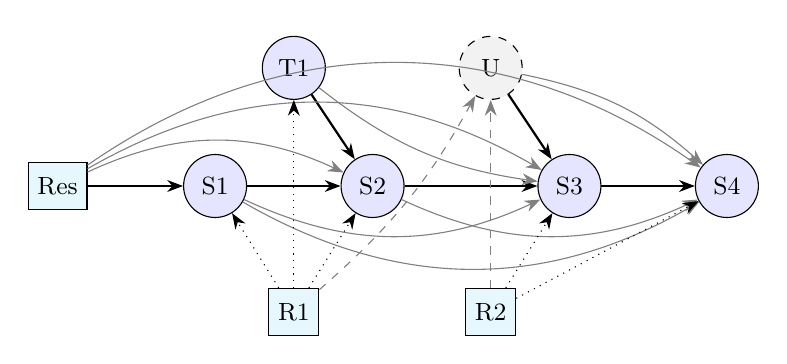
\begin{tikzpicture}[font=\small, >={Stealth[length=2mm]},
  st/.style={circle, draw, fill=blue!10, minimum size=8mm, inner sep=0pt},
  lat/.style={circle, draw, dashed, fill=gray!10, minimum size=8mm, inner sep=0pt},
  rn/.style={rectangle, draw, fill=cyan!10, minimum size=6mm}]
\node[rn] (res) at (0,0) {Res};
\node[st] (s1) at (2,0) {S1};
\node[st] (t1) at (3,1.5) {T1};
\node[st] (s2) at (4,0) {S2};
\node[lat] (u) at (5.5,1.5) {U};
\node[st] (s3) at (6.5,0) {S3};
\node[st] (s4) at (8.5,0) {S4};
\node[rn] (r1) at (3,-1.6) {R1};
\node[rn] (r2) at (5.5,-1.6) {R2};
\foreach \a/\b in {res/s1,s1/s2,t1/s2,s2/s3,u/s3,s3/s4} \draw[->, thick] (\a) -- (\b);
\draw[->, gray, bend left=25] (res) to (s2);
\draw[->, gray, bend left=30] (res) to (s3);
\draw[->, gray, bend left=35] (res) to (s4);
\draw[->, gray, bend right=25] (s1) to (s3);
\draw[->, gray, bend right=30] (s1) to (s4);
\draw[->, gray, bend right=25] (s2) to (s4);
\draw[->, gray, bend right=15] (t1) to (s3);
\draw[->, gray, bend left=15] (u) to (s4);
\draw[->, dotted] (r1) -- (s1); \draw[->, dotted] (r1) -- (s2); \draw[->, dotted] (r1) -- (t1);
\draw[->, dotted] (r2) -- (s3); \draw[->, dotted] (r2) -- (s4);
\draw[->, dashed, gray] (r1) to[bend right=10] (u); \draw[->, dashed, gray] (r2) -- (u);
\end{tikzpicture}
\caption{Directed graph used by the delay-attention layer. Black: physical river links. Grey:
transitive edges from every upstream source to every downstream station, each with its own lag
window, so the reach of one layer covers the whole basin. Dotted: rainfall-to-catchment edges
(initial assignment from gauge locations, A10). Dashed: the latent node U has no sensor, and its
sequence is produced from R1 and R2 by the latent-inflow encoder. All edges point downstream (A7).}
\label{fig:graph}
\end{figure}

%----------------------------------------------------------------------
\section{Assumptions}
%----------------------------------------------------------------------
\textbf{Supplied facts (not assumptions).} 10-minute water levels at S1--S4 and T1; rainfall at
R1 and R2 with timestamps and gauge locations; recorded reservoir releases and announced future
schedules with announcement and effective times; station locations, river connectivity and
along-river distances. A monitored tributary (T1) joins between S1 and S2 and an unmonitored one
between S2 and S3. Stations are unevenly spaced, travel times vary with conditions, precise
travel times and the unmonitored inflow are not supplied, and future rainfall and future levels are
unknown at issuance. Everything below is an assumption made because the brief leaves it open.

\subsection*{Unspecified data conditions}
\begin{description}[leftmargin=0.9cm, style=nextline]
\item[A1 Record length.] At least three years of history are available for all sources and include
several flood seasons. \emph{Why reasonable:} authorities normally keep multi-year telemetry archives.
\emph{Effect on design:} enough events for a small ($\approx$0.3\,M parameter) model, but not for a large
one; data are split chronologically (oldest years train, next season validation, most recent season
test) so that no future information leaks into training.
\item[A2 Reporting delays.] Level telemetry usually arrives within one 10-minute interval but can be up
to 30\,min late; rain gauges report with up to 20\,min delay; reservoir releases are logged within
10\,min. \emph{Why:} typical of radio/GSM telemetry. \emph{Effect:} every input is built ``as of''
$\tau$ with an explicit \emph{age} feature, and training replays these delays (Section~5).
\item[A3 Measurement quality.] Gauges share a common datum; level noise is a few centimetres;
occasional spikes and flat-lines occur. \emph{Why:} standard for pressure/radar gauges.
\emph{Effect:} range and rate-of-change checks flag bad readings, which are then treated as missing.
\item[A4 Missingness.] Gaps are sporadic (a few \% of readings) and occasionally last hours; no
station is missing for most of the record. \emph{Why:} sensors are maintained. \emph{Effect:} masks
plus simple filling suffice; a permanently failed station needs retraining or a fallback model.
\item[A5 Release semantics.] A release value (m$^3$/s) holds from its effective time until the next
record (step function). Announced schedules are usually followed but can be revised or deviate
(gate errors, emergency spills). \emph{Why:} how gate operations are logged. \emph{Effect:} scheduled
and actual releases are separate inputs (Sections~4--5).
\item[A6 Issuance timing.] Forecasts are issued at the grid times
($\ldots$, hh:00, hh:10, $\ldots$) after a short collection cut-off (2\,min), and the target is the
level recorded at $\tau+60$\,min. \emph{Why:} matches the 10-minute logging. \emph{Effect:} defines
$\tau$ and the alignment grid (Section~3).
\end{description}

\subsection*{River dynamics the model assumes}
\begin{description}[leftmargin=0.9cm, style=nextline]
\item[A7 Downstream-only propagation.] There is no tidal influence or significant backwater from
downstream structures on S1--S4. \emph{Why:} an inland river below a reservoir. \emph{Effect:} graph
edges point downstream only, which removes spurious paths and is a strong inductive bias.
\item[A8 Bounded, state-dependent travel times.] The travel time of a flood wave over a distance
$d_{ij}$ is $d_{ij}/c$, with wave celerity $c$ between $c_{\min}=0.5$ and $c_{\max}=4$\,m/s, and $c$
grows with discharge (faster in floods). \emph{Why:} the typical range for lowland and mid-gradient
rivers. \emph{Effect:} edge $j\to i$ may only use lags in
$\Lambda_{ij}=[\lfloor d_{ij}/(c_{\max}\Delta)\rfloor,\ \lceil d_{ij}/(c_{\min}\Delta)\rceil+3]$
(10-minute steps, with a margin). Within $\Lambda_{ij}$ the weights are learned and depend on the
current level (Section~4). Travel time is therefore learned, but physically impossible lags are
excluded.
\item[A9 Smooth, monotone response.] Over one hour, the level change at a station is dominated by
recent upstream changes, routed inflows and local rainfall-runoff. More inflow never lowers the
level downstream. \emph{Why:} mass conservation in an open channel. \emph{Effect:} we predict the
change over persistence (residual form), and an optional penalty keeps the median forecast
non-decreasing in the scheduled release.
\item[A10 Rainfall representativeness.] From the gauge locations, R1 mainly drains to S1, S2 and T1,
and R2 to the unmonitored tributary, S3 and S4. \emph{Why:} nearest-catchment assignment.
\emph{Effect:} initial rainfall-to-node edges. Their weights are learned, so a wrong guess is
down-weighted by the data.
\item[A11 Stationary channel.] No major change of the river bed or the level--flow relation occurs within the
record, and the authority reports such changes. \emph{Why:} short record. \emph{Effect:} one model
for the whole record, with drift monitoring triggering retraining.
\item[A12 Rain after issuance is secondary within one hour.] Rain that has fallen by $\tau$ dominates
the one-hour response, and rain falling after $\tau$ matters mainly for the fastest catchments.
\emph{Why:} runoff concentration times usually exceed one hour. \emph{Effect:} no rainfall forecast
is required, and the remaining effect is absorbed by the upper quantile (Section~6).
\end{description}

%----------------------------------------------------------------------
\section{Forecasting task and data specification}
%----------------------------------------------------------------------
\textbf{Issuance time.} $\tau$ is a 10-minute grid time (A6). A forecast is issued every
$\Delta=10$\,min using only the data that have \emph{arrived} by $\tau$.

\textbf{History window.} $L=72$ steps (12\,h): $\{\tau-71\Delta,\dots,\tau\}$. Twelve hours is longer
than the largest admissible travel time from the reservoir to S4 (A8) plus the rainfall-runoff
response, so the causes of everything that arrives at a station within the next hour lie inside
the window.

\textbf{Horizon.} One hour ahead, i.e.\ $h=6$ steps. The target time is $\tau^{+}=\tau+6\Delta$. The
intermediate steps $\tau+\Delta,\dots,\tau+5\Delta$ are predicted as auxiliary outputs during
training only, to give more training signal. The service publishes $\tau^{+}$.

\textbf{Outputs.} For each station S1--S4, the 10\,\%, 50\,\% (point forecast) and 90\,\% quantiles of the
water level at $\tau^{+}$, in metres above the gauge datum.

\begin{table}[H]
\centering\small
\caption{Inputs and outputs for one batch. $B$ is the batch axis: each sample is one issuance
time $\tau$, and the samples of a batch come from different dates. $L=72$, $H=6$; $E$ is the
number of directed edges.}
\label{tab:data}
\begin{tabularx}{\textwidth}{@{}p{2.6cm}p{2.5cm}Xp{3.6cm}@{}}
\toprule
Tensor & Dimensions & Axis meanings & Time coverage / timestamps\\
\midrule
$\mathbf{Y}^{\mathrm{hist}}$ levels & $B\times5\times L\times4$ & batch; node (S1, S2, S3, S4, T1);
history step; feature (level, 10-min level change, valid mask, age of last valid reading) &
grid times $\tau-71\Delta\ldots\tau$, readings that arrived by $\tau$\\
$\mathbf{P}$ rainfall & $B\times2\times L\times3$ & batch; gauge (R1, R2); history step; feature
(rain in the 10-min bin, valid mask, age) & bins $(\tau-(l{+}1)\Delta,\ \tau-l\Delta]$ by gauge
timestamp, $l=0..71$\\
$\mathbf{Q}^{\mathrm{past}}$ releases & $B\times1\times L\times4$ & batch; reservoir; history step;
feature (actual release, release scheduled for that time, valid mask, age) & grid times
$\tau-71\Delta\ldots\tau$, by effective time\\
$\mathbf{Q}^{\mathrm{sch}}$ schedule & $B\times1\times H\times2$ & batch; reservoir; future step;
feature (scheduled release, time since announcement) & $\tau+\Delta\ldots\tau+6\Delta$ by effective
time; only schedules announced at or before $\tau$\\
$\mathbf{C}$ calendar & $B\times L\times2$ & batch; history step; (sin, cos of day of year) & as history\\
$\mathbf{A}$, $\mathbf{e}$ static graph & $E\times2$, $E\times4$ & edge; (source, target) / edge features
(distance, $\min\Lambda_{ij}$, $\max\Lambda_{ij}$, edge type). Shared by all samples (no batch axis) &
time-invariant\\
\midrule
$\hat{\mathbf{Y}}$ forecast & $B\times4\times3$ & batch; station (S1--S4); quantile (0.1, 0.5, 0.9)
& $\tau^{+}=\tau+6\Delta$\\
$\hat{\mathbf{Y}}^{\mathrm{aux}}$ (training only) & $B\times4\times H\times3$ & batch; station; future
step; quantile & $\tau+\Delta\ldots\tau+6\Delta$\\
$\mathbf{Y}$ target & $B\times4\times H$ (+ mask) & batch; station; future step & $\tau+\Delta\ldots
\tau+6\Delta$ (the service is scored on the last step)\\
\bottomrule
\end{tabularx}
\end{table}

\textbf{Alignment across sampling times.} All sources are mapped onto the same
issuance-anchored grid before encoding.
\begin{itemize}[leftmargin=*,itemsep=1pt]
\item \emph{Levels} (S1--S4, T1) are already on the grid. A slot holds a reading only if the
reading has arrived by $\tau$. Otherwise it is masked and filled with the last valid value, and
its \emph{age} records how stale that value is.
\item \emph{Rainfall} arrives as timestamped events or irregular totals. It is summed into 10-minute bins
by \emph{measurement} time. Bins whose data have not yet arrived are masked.
\item \emph{Releases} are step functions (A5), sampled at each grid time by their \emph{effective}
time. The release that was scheduled for each past time is kept as a second channel, so the network
can see how far the schedule and the actual release have differed.
\item \emph{Announced schedule}: an ``as-of'' join takes, for each future step, the most recent
schedule whose \emph{announcement} time is $\le\tau$. Later announcements are invisible, exactly as
in operation, and a schedule announced before $\tau$ but effective after $\tau+60$\,min is irrelevant.
\end{itemize}

\textbf{Alignment across locations.} Locations are not interpolated onto a spatial grid. Each
sensor is a graph node (S1--S4, T1), or feeds one (R1, R2 feed their catchment nodes and the latent
node U). River geometry enters through the edge features and the lag windows $\Lambda_{ij}$
derived from along-river distances (A8). Encoders are shared across sensors of the same type, a
learned node embedding tells the sensors apart, and per-source linear projections bring every input
to the same width $d$ before the graph layer combines them (Figure~\ref{fig:arch}).

\textbf{Information available at issuance:} all history up to $\tau$ that has arrived, the latest
announced release schedule up to $\tau+60$\,min, and the static data. \textbf{Not available:} future
rainfall, future levels (including any reading not yet delivered), the unmonitored tributary inflow,
and exact travel times.

%----------------------------------------------------------------------
\section{Model computations and design justification}
%----------------------------------------------------------------------
\textbf{Notation.} Nodes $\mathcal{V}=\{\mathrm{Res},\mathrm{T1},\mathrm{U},\mathrm{S1},\mathrm{S2},\mathrm{S3},\mathrm{S4}\}$;
rain gauges $\mathcal{G}=\{\mathrm{R1},\mathrm{R2}\}$; stations $\mathcal{S}=\{\mathrm{S1},\dots,\mathrm{S4}\}$.
$\mathcal{N}^{\uparrow}(i)$ is the set of sources with an edge into $i$ (Figure~\ref{fig:graph}).
$x_{j,t}$ is the aligned feature vector of source $j$ at grid step $t$ (Table~\ref{tab:data}).
$y_i(t)$ is the level of station $i$, $\tau^{+}=\tau+6\Delta$, and lags $\ell$ are counted in
10-minute steps \emph{back from the target time} $\tau^{+}$.

\subsection*{Main blocks}
\textbf{(1) Per-source causal encoders} (learned). A causal dilated temporal convolution (TCN:
kernel 3, dilations $1,2,\dots,32$, receptive field 127 steps $\ge L$), a source-type-specific
projection to width $d$, and a learned node embedding $\mathbf{p}_j$:
\begin{equation}
\mathbf{z}_{j,t}=W^{(s)}_{\mathrm{proj}}\,\mathrm{TCN}^{(s)}\!\big(x_{j,\le t}\big)+\mathbf{p}_j\in\mathbb{R}^{d},\qquad t\le\tau ,
\end{equation}
where $s\in\{\text{level},\text{rain},\text{release}\}$ and the mask and age are input channels.
Causality guarantees that $\mathbf{z}_{j,t}$ never sees data after $t$. The reservoir sequence is
extended into the future with the announced schedule:
$\mathbf{z}_{\mathrm{Res},\tau+h}=\mathrm{MLP}\big([Q^{\mathrm{sch}}_{\tau+h},a_{\tau+h},h]\big)$ for $h=1,\dots,6$.
The latent node U has no sensor. Its sequence is a learned rainfall-runoff transform of both
gauges, $\mathbf{z}_{\mathrm{U},t}=\mathrm{TCN}^{(\mathrm{U})}\big(x_{\mathrm{R1},\le t},x_{\mathrm{R2},\le t}\big)+\mathbf{p}_{\mathrm{U}}$,
and it is trained only through its effect on S3 and S4.

\textbf{(2a) Delay-attention layer} (learned weights on a physically restricted support). For an
edge $j\to i$, the admissible lags are those in the travel-time window $\Lambda_{ij}$ (A8) that refer
to known data:
\begin{equation}
\mathcal{A}_{ij}=\big\{\ell\in\Lambda_{ij}:\ \tau^{+}-\ell\Delta\le\tau\big\}\ \ (\ell\ge6)\ \text{for observed sources},\qquad
\mathcal{A}_{\mathrm{Res},i}=\Lambda_{\mathrm{Res},i}\ \text{(schedule known)} .
\end{equation}
If $\Lambda_{ij}$ lies entirely below 6, i.e.\ the travel time is under one hour, then
$\mathcal{A}_{ij}=\{6,\dots,6+3\}$: the most recent upstream state, whose TCN encoding contains
its trend. The message is a soft choice of the arrival lag:
\begin{align}
\alpha_{ij,\ell}&=\operatorname*{softmax}_{\ell\in\mathcal{A}_{ij}}
\frac{\big(W_Q\mathbf{z}_{i,\tau}\big)^{\!\top}W_K\big[\mathbf{z}_{j,\tau^{+}-\ell}\,\Vert\,\mathbf{e}_{ij}\,\Vert\,\phi(\ell)\big]}{\sqrt d},
&\mathbf{m}_{ij}&=\sum_{\ell\in\mathcal{A}_{ij}}\alpha_{ij,\ell}\,W_V\mathbf{z}_{j,\tau^{+}-\ell},\\
\beta_{ij}&=\operatorname*{softmax}_{j\in\mathcal{N}^{\uparrow}(i)}\mathbf{w}_\beta^{\!\top}\tanh\!\big(W_\beta[\mathbf{z}_{i,\tau}\Vert\mathbf{m}_{ij}\Vert\mathbf{e}_{ij}]\big),
&\mathbf{h}^{(1)}_{i}&=\mathrm{LN}\Big(\mathbf{z}_{i,\tau}+\mathrm{MLP}\big(\textstyle\sum_{j\in\mathcal{N}^{\uparrow}(i)}\beta_{ij}\mathbf{m}_{ij}\big)\Big),
\end{align}
with $\phi(\ell)$ a learned lag embedding. The query $\mathbf{z}_{i,\tau}$ encodes the current
state of the receiving station (its level and trend), so in high flow the attention moves to
shorter lags. \emph{Changing travel times} are thus a learned mapping, and only the window
$\Lambda_{ij}$ is a physical assumption. The weights $\beta_{ij}$ decide how much each upstream source
contributes (for example T1 versus S1 for S2).

\textbf{(2b) Downstream message passing on node states} (learned). One more layer on the
current node states,
$\mathbf{h}^{(2)}_{i}=\mathrm{LN}\big(\mathbf{h}^{(1)}_{i}+\mathrm{MLP}\big(\sum_{j\in\mathcal{N}^{\uparrow}(i)}\gamma_{ij}W_M\mathbf{h}^{(1)}_{j}\big)\big)$
with attention weights $\gamma_{ij}$ computed like $\beta_{ij}$. It lets a station use what
upstream nodes have already worked out about themselves. For example, S3 receives the summary of U
(rain-driven inflow) and of S2 (its own upstream context).

\textbf{(3) Fusion and forecast mapping.} For each station $i\in\mathcal{S}$, a GRU over its own
encoded history gives $\mathbf{s}_i$. A gate decides how far to trust the graph context:
\begin{equation}
\mathbf{g}_i=\sigma\big(W_g[\mathbf{s}_i\Vert\mathbf{h}^{(2)}_i]\big),\qquad
\mathbf{f}_i=\mathbf{g}_i\odot\mathbf{h}^{(2)}_i+(1-\mathbf{g}_i)\odot\mathbf{s}_i .
\end{equation}
The head predicts the \emph{change} over persistence (A9), scaled by $\sigma_i$, the training-set
standard deviation of one-hour changes at station $i$, for each step $h=1..6$:
\begin{equation}
\hat y_{i,0.5}(\tau+h\Delta)=y_i(\tau^{\ast}_i)+\sigma_i\,\mathbf{w}_{h}^{\top}\mathbf{f}_i,\qquad
\hat y_{i,0.5\pm0.4}=\hat y_{i,0.5}\pm\sigma_i\,\mathrm{softplus}\big(\mathbf{w}^{\pm\top}_{h}\mathbf{f}_i\big),
\end{equation}
where $y_i(\tau^{\ast}_i)$ is the last valid level. The softplus offsets prevent quantile crossing.
The published forecast is $h=6$.

\textbf{(4) Training objective.}
\begin{equation}
\mathcal{L}=\frac{1}{|B|}\sum_{b\in B}\sum_{i\in\mathcal{S}}\sum_{h=1}^{6}\omega_{b}\,w_h\,M_{b,i,h}
\sum_{q\in\{0.1,0.5,0.9\}}\rho_q\!\left(\frac{y_i(\tau_b+h\Delta)-\hat y_{i,q}(\tau_b+h\Delta)}{\sigma_i}\right)
+\lambda\,\mathcal{R}_{\mathrm{mono}},
\end{equation}
with the pinball loss $\rho_q(r)=\max(qr,(q-1)r)$; $w_6=1$ and $w_{h<6}=0.2$ (auxiliary steps);
$M_{b,i,h}$ masking missing targets; $\omega_b=3$ for samples whose target exceeds the 95th
percentile level (floods matter most for preparedness) and 1 otherwise; and the optional monotonicity
penalty $\mathcal{R}_{\mathrm{mono}}=\mathbb{E}\big[\mathrm{ReLU}\big(-\partial\hat y_{i,0.5}/\partial Q^{\mathrm{sch}}\big)\big]$ (A9).
Training uses chronological splits (A1), AdamW, early stopping on the validation pinball loss, and the
missing/delay augmentation of Section~5.

\subsection*{How each driver reaches a forecast}
\begin{itemize}[leftmargin=*,itemsep=1pt]
\item \textbf{Upstream conditions.} S$k$ receives every upstream station through its own delay edge,
at lags matching the travel time. These edges carry most of the one-hour signal at S2--S4.
\item \textbf{Tributaries.} T1 is a node with lag windows into S2 (and onward to S3 and S4). The
unmonitored tributary is the latent node U. It is driven by rainfall, mostly R2 (A10), and is
implicitly calibrated by whatever part of S3's change S2 cannot explain, because this is the only
way the loss can use it.
\item \textbf{Rainfall.} Edges from R1 and R2 to their catchment nodes use lag windows covering
runoff times (0--6\,h). Rain therefore acts directly as local runoff and indirectly through the
upstream nodes and U.
\item \textbf{Reservoir releases.} Past releases act through the Res node. Announced releases act
through its future extension, and the lag window lets a release effective within the hour affect S1
before $\tau^{+}$ if its travel time is short enough (Section~5).
\end{itemize}

\subsection*{Physical assumptions versus learned mappings}
\textbf{Physical (fixed by design):} downstream edge directions (A7); lag windows from distances and
celerity bounds (A8); the residual-over-persistence form and the monotonicity prior (A9); the
existence of an unobserved inflow node between S2 and S3; and causality (no data after $\tau$, except
announced releases). \textbf{Learned:} travel time as a function of state (the lag weights $\alpha$), the
strength and attenuation of each influence ($W_V$, $\beta$, $\gamma$), the rainfall-runoff response,
the latent tributary state, the gating between own history and context, and the uncertainty
(quantiles). We do not hard-code a hydraulic model such as Muskingum or Saint-Venant, because its
parameters are not supplied; Section~6 describes how one can be added.

\subsection*{Justification of the main choices}
\begin{enumerate}[leftmargin=*,itemsep=1pt]
\item \textbf{Reach.} A forecaster cannot use information that is outside its reach, measured in hops
and in time (as the companion notebook shows). Transitive delay edges connect every upstream source
to every station within one layer, and the 12\,h window covers the longest admissible travel time.
A stack of single-hop layers would need at least four layers to bring reservoir information to S4.
\item \textbf{Bounded lag attention} is cheap, interpretable (the attention peak is an estimated
travel time, so the committee can inspect it), causal, and cannot use physically impossible lags.
Compared with full space-time attention it has few free parameters, which suits a few years of
data (A1).
\item \textbf{Separate encoders projected to a common width} handle the different sampling
(events versus grid) and feature sets of the sources (Figure~\ref{fig:arch}).
\item \textbf{Residual forecasting with gating} keeps persistence as a safe default. If upstream
inputs are missing, the gate falls back to the station's own history.
\item \textbf{Quantile outputs} give decision-makers an interval that can be read directly, for
example ``a 10\,\% chance that S3 exceeds the warning level within the hour''.
\end{enumerate}

%----------------------------------------------------------------------
\section{Operation and exceptional conditions}
%----------------------------------------------------------------------
\textbf{(i) Missing observations.}
\begin{itemize}[leftmargin=*,itemsep=1pt]
\item Every value carries a mask bit and an age (Table~\ref{tab:data}). Missing levels are filled
with the last valid value and missing rain with zero, so the network can see that the value is
stale and is not misled by the fill.
\item Training randomly drops single readings, whole hours and entire stations (10--20\,\% of
samples), so the model learns to rely on neighbours, rainfall and the latent node when a sensor is
silent. The gate in block (3) learns when the station's own history cannot be trusted.
\item The forecast anchor $y_i(\tau^{\ast}_i)$ is the last valid reading. If a station has been
silent for more than one hour, its forecast is still issued from upstream information but is
flagged \emph{degraded}, and its quantile interval is wider (learned from the masked training
samples).
\item Missing targets are excluded from the loss ($M_{b,i,h}$) and never imputed for training.
\end{itemize}

\textbf{(ii) Delayed observations.}
\begin{itemize}[leftmargin=*,itemsep=1pt]
\item Inputs are always assembled \emph{as of} $\tau$ (A2): a reading that has not arrived is
treated as missing, with its age, and the system does not wait for it.
\item When the late reading arrives, the next issuance ten minutes later uses it automatically,
because the history window is rebuilt every cycle. Published forecasts are not rewritten. Each is
archived with a snapshot of the data available when it was made, so later evaluation reflects what
the system actually knew.
\item Training replays the empirical delay distribution, so the model is trained with the same
information it will have in operation. Training on the complete, cleaned archive would overstate
accuracy.
\end{itemize}

\textbf{(iii) Announced future releases.}
\begin{itemize}[leftmargin=*,itemsep=1pt]
\item The latest schedule announced at or before $\tau$ is placed on the future grid
$\tau+\Delta..\tau+6\Delta$ by \emph{effective} time (as-of join, Section~3) and enters through the
reservoir's future extension. It is the only input from after $\tau$.
\item A ``time since announcement'' feature lets the model learn that recent announcements are
more reliable than old ones.
\item If no schedule covers part of the horizon, the last actual release is held (A5) and a mask
bit marks the gap.
\item A release takes time to reach a station. Only S1, and in floods possibly S2, can feel a release
effective within the hour before $\tau^{+}$. The lag windows encode this, so a change in the
announced schedule cannot implausibly affect S4 within the hour.
\end{itemize}

\textbf{(iv) Differences between scheduled and actual releases.}
\begin{itemize}[leftmargin=*,itemsep=1pt]
\item For past steps, the model always sees the \emph{actual} release, plus the release that had
been scheduled for that time as a separate channel ($\mathbf{Q}^{\mathrm{past}}$). It therefore
learns how schedules and actual releases historically differ, and how much to trust them.
\item As soon as a measured release departs from the schedule, the measured value replaces the
schedule for all elapsed steps at the next issuance (at most ten minutes later). The current
deviation, actual minus scheduled, is visible in the input and informs how much the remaining
schedule is trusted.
\item A deviation above an operational threshold triggers an operator alert, a wider interval, and
an optional scenario forecast with the alternative release, which costs only one more forward pass.
\item Training perturbs announced schedules (random offsets and time shifts relative to the actual
releases), so the model does not over-trust announcements.
\end{itemize}

\textbf{Feasibility every ten minutes.} One forward pass handles 7 nodes, 2 gauges, 72 history
steps, about 25 edges with at most 40 admissible lags each, and $d=64$. That is about $10^{7}$
multiply-adds, i.e.\ a few milliseconds on one CPU core. Assembling the inputs takes a handful of
database queries. Even an ensemble of five models plus a few release scenarios stays well under one
second, which leaves almost all of the 10-minute cycle for data collection, quality control and
dissemination. Training is offline (for example monthly, or after a reported channel change, A11)
and takes minutes to hours on a single GPU.

%----------------------------------------------------------------------
\section{Uncertainty, limitations, and additional information}
%----------------------------------------------------------------------
\subsection*{Uncertainties and limitations}
\begin{table}[H]
\centering\small
\begin{tabularx}{\textwidth}{@{}p{2.9cm}XX@{}}
\toprule
Uncertainty / limitation & Forecast impact & Response, or what remains unresolved\\
\midrule
Unmonitored tributary &
Inflow between S2 and S3 is unknown. When it carries a flood that S2 does not see, S3 and then S4
are under-predicted. &
Latent node U driven by R1/R2 and calibrated by the unexplained part of S3's change; wider
intervals at S3/S4. \emph{Unresolved:} a local storm missed by R2 is invisible until S3 itself
starts to rise.\\
Changing travel times &
Fixed lags would arrive early in low flow and late in floods, mis-timing the peak. &
State-dependent delay attention within physical windows (A8). \emph{Unresolved:} floods beyond the
training range may exceed the assumed celerity bounds.\\
Travel time shorter than the horizon &
For short reaches (Res$\to$S1, possibly S1$\to$S2), the upstream signal that will arrive by
$\tau^{+}$ has not been measured yet at $\tau$. &
The model extrapolates the latest upstream trend (TCN state), and for S1 it uses the announced
schedule. The remaining uncertainty is reflected in wider intervals.\\
Future rainfall &
Rain after $\tau$ can raise levels within the hour in fast catchments (A12). &
Absorbed by the upper quantile. Resolvable with a rainfall nowcast (request 3).\\
Release deviations &
Over-trusting a schedule biases S1 and S2. &
Separate scheduled and actual channels, deviation feature, alerts (Section~5).\\
Sparse rain gauges &
Two gauges cannot capture spatially variable rain. &
Learned catchment weights. \emph{Unresolved} without radar or more gauges.\\
Rare extremes &
Few floods in a short record (A1). The model may under-predict peaks, which are the costliest errors. &
Flood re-weighting, residual form, conservative 90\,\% quantile, and validation on every historical
flood event separately.\\
Distribution shift &
Channel or level--flow changes (A11), new reservoir rules. &
Drift monitoring of residuals and retraining.\\
Model uncertainty &
Aleatoric noise and epistemic error from limited data. &
Quantile loss (aleatoric), an ensemble of five seeds (epistemic), and a check that the 10--90\,\%
interval contains about 80\,\% of test outcomes.\\
\bottomrule
\end{tabularx}
\end{table}

\subsection*{Additional information requests}
Each item is optional. Without any of them the system remains usable, with lower accuracy or wider
intervals.
\begin{enumerate}[leftmargin=*,itemsep=2pt]
\item \textbf{Level--flow (rating) curves or discharge at S1--S4 and T1.} These convert levels to
flows and allow mass-balance features. The S3 inflow not explained by S2 directly estimates the
unmonitored tributary. \emph{Without it:} usable; the model works on levels.
\item \textbf{Any measurements on the unmonitored tributary}, even a temporary gauge for one season.
These would calibrate the latent node U. \emph{Without it:} usable; U stays latent.
\item \textbf{Rainfall nowcasts (radar, 0--1\,h) and additional gauges.} These would reduce the
largest remaining error, from rain after issuance and between gauges. \emph{Without it:} usable (A12).
\item \textbf{Cross-sections or historical travel-time studies.} These give tighter lag windows
than the generic celerity bounds. \emph{Without it:} usable, using A8.
\item \textbf{Telemetry metadata} (reporting delays, maintenance logs, sensor changes). These make
the delay simulation and quality flags realistic. \emph{Without it:} usable, with A2--A4.
\item \textbf{Reservoir operating rules and the history of schedule revisions.} These would help
model release deviations better. \emph{Without it:} usable.
\item \textbf{Reservoir inflow and reservoir level.} These would help anticipate spills before they
are announced. \emph{Without it:} usable.
\end{enumerate}

\subsection*{Treatment of physical relationships and uncertainty}
No separate physical simulator is required. Physics enters through A7--A9: edge directions, lag
windows and the residual and monotone form. Uncertainty enters through quantile outputs and a
small ensemble. If rating curves and channel data are supplied (requests 1 and 4), a Muskingum
routing of the reservoir release and of T1 can be run alongside, and its routed flow at each station
added as an input channel. The network then learns a correction to the physical model (hybrid
modelling), which matters most for floods outside the training range.


\newpage
%======================================================================
\part*{Question 2 -- Motion or Memory?}
\addcontentsline{toc}{part}{Question 2 -- Motion or Memory?}
%======================================================================
\setcounter{section}{0}
% Unique hyperlink targets for Question 2's restarted section, table and figure numbers.
\renewcommand{\theHsection}{q2.\arabic{section}}
\renewcommand{\theHtable}{q2.\arabic{table}}
\renewcommand{\theHfigure}{q2.\arabic{figure}}
% Question 2 -- Motion or Memory?  (included by main.tex)
\setcounter{table}{0}
\setcounter{figure}{0}
\newcommand{\qa}[1]{\paragraph{Q2.#1}}
\newcommand{\Ex}[1]{E^{(#1)}}

\paragraph{Conventions.} Every table entry for a learned model is \emph{mean (seed 0, seed 1)};
Blank and Copy-last are deterministic and get a single value. Errors have three significant figures,
and values below $10^{-3}$ use scientific notation. All model results are on the 1,000 test videos
(9,000--9,999) at $t=1$, unless stated otherwise. Code: \texttt{Question2/} in the repository
(\texttt{Question2/README.md} lists the command that produces each table and figure).

\paragraph{Hardware and timing.} Everything was run on one laptop CPU: AMD Ryzen~5 7430U
(6 cores, 12 threads), 15\,GB RAM, no GPU, Linux 7.2, Python~3.14, PyTorch~2.15.0 (CPU build).
Training used 12 threads, with one run at a time. Inference was timed with PyTorch's default 6 threads,
following the protocol in the handout (batch 32, \texttt{eval()}, \texttt{no\_grad()}, all 1,000 test videos).
\emph{Note on model~A, seed~0:} its first five epochs (303, 276, 225, 221 and 227\,s) ran while other
applications and package installation shared the CPU, and training was resumed from checkpoints after
interruptions (resuming reproduces the uninterrupted weights bit for bit). Its reported 30-epoch mean of
210\,s is the measured value. Its epochs 6--30 average 202\,s, the same as the other baseline-architecture
runs (202--205\,s). The same applies to \emph{model~C, seed~0}: its epochs 4--13 (220--275\,s, mean 242\,s)
shared the CPU with other work and two interruptions, so its measured mean is 216\,s; its other 20 epochs
average 203\,s. Model~D and D+B take about 60\,s per epoch.

%======================================================================
\section{Setup}
%======================================================================
The videos are split by dataset index (0--7,999 train, 8,000--8,999 validation, 9,000--9,999 test)
and scaled to $[0,1]$. All checks in Table~\ref{tab:q2-t1} call the same transformation and window
functions that the experiments use (\texttt{q2/data.py}), and every row matches.

\begin{table}[H]
\centering\small
\caption{Checks of the transformation and window functions.}
\label{tab:q2-t1}
\begin{tabular}{lll}
\toprule
Check & Expected & Yours \\
\midrule
(a) max$|$M(M(x)) - x$|$ & 0 & 0 (torch.equal=True) \\
(b) max$|$R$^4$(x) - x$|$ & 0 & 0 (torch.equal=True) \\
(c) max$|$M R M(x) - R$^{-1}$(x)$|$ & 0 & 0 (torch.equal=True) \\
(d) bright pixel of M(p) & (7, 10, 43) & (7, 10, 43) \\
(e) bright pixel of R(p) & (7, 43, 10) & (7, 43, 10) \\
(f) 1x input / target frames & 1-5 / 6-10 & 1, 2, 3, 4, 5 / 6, 7, 8, 9, 10 \\
(g) 2x input / target frames & 1, 3, 5, 7, 9 / 11, 13, 15, 17, 19 & 1, 3, 5, 7, 9 / 11, 13, 15, 17, 19 \\
(h) 3x input / target frames & 1, 4, 7, 10, 13 / 16, 19 & 1, 4, 7, 10, 13 / 16, 19 \\
\bottomrule
\end{tabular}

\end{table}

\begin{figure}[H]
\centering
\includegraphics[width=\linewidth]{fig1_flow.png}
\caption{Farneback optical flow on the first 50 training videos (950 consecutive frame pairs).
103,050 pixels are kept (intensity $>0.2$ in both frames, flow magnitude $>0.5$\,px).
(a) Flow direction $\theta=\mathrm{atan2}(-d_y,d_x)$ in 18 bins of $20^\circ$, as the fraction of kept pixels;
the dashed line is the uniform level $1/18$.
(b) Flow speed in px/frame, as the fraction of kept pixels; the median is 3.32\,px/frame (dashed line).}
\label{fig:q2-f1}
\end{figure}

\qa{1} \emph{Directions.} Every $20^\circ$ bin holds between 2.6\,\% and 8.2\,\% of the kept pixels
(uniform: 5.6\,\%). No direction is missing; the unevenness comes from having only about 100 digit
trajectories (50 videos, two digits each). A mirror maps $\theta\mapsto180^\circ-\theta$, and a $90^\circ$
rotation maps $\theta\mapsto\theta+90^\circ$. So mirroring or rotating every training video would only
reorder the bars of Figure~\ref{fig:q2-f1}(a). Applying these maps to the measured histogram moves it by a
total-variation distance of 0.132 (mirror) and 0.200 (rotation), comparable to its distance from uniform
(0.110). Every direction in a mirrored or rotated video is therefore a direction the model has seen in
at least 2.6\,\% of its training pixels, so the trajectories themselves are familiar. Only their
frequencies change, and rotation reshuffles them more than mirroring.
\emph{Speeds.} The median speed is 3.32\,px/frame (interquartile range 3.00--3.89, 95th percentile 4.32,
99th 4.67). At 2$\times$ the digits move about 6.6\,px per observed frame (95th percentile 8.6), and at
3$\times$ about 10.0\,px (95th percentile 13.0). Both are far outside the training range, where almost no
pixel moves more than 5\,px.
\emph{Overlap.} Farneback assumes that a pixel keeps its brightness as it moves and that motion is locally
smooth. Where two digits overlap, both assumptions fail: the pixel saturates, and two motions share one
neighbourhood. The flow there is a blend of the two directions and is usually too short, so it adds a
little mass to the slow tail of Figure~\ref{fig:q2-f1}(b) (with bounces and digit edges) and smears a few
pixels across directions. Overlaps cover a small fraction of the kept pixels and do not remove any
direction, so they can slightly lower the median speed and smooth the histogram, but cannot change
either answer above.

\qa{2} \emph{Mirror}: changes the appearance (a mirrored 2 is not a 2) and relabels directions
($\theta\mapsto180^\circ-\theta$), with speeds unchanged; every resulting direction occurs in training.
\emph{Rotation}: changes the appearance even more (digits lie on their side, so vertical and horizontal
strokes swap) and relabels directions ($\theta\mapsto\theta+90^\circ$), again with speeds unchanged.
\emph{Speed-up}: leaves the appearance untouched and changes only the motion statistics. Every
displacement is multiplied by $k$, beyond anything seen in training, and bounces fall between observed
frames more often. Together they form a controlled experiment. The true dynamics are invariant to all
three, and the correct transformed future $T(Y)$ is known exactly, so any failure belongs to the model,
not the task. Each transformation also changes a different factor: speed-up isolates unfamiliar
\emph{motion} at fixed appearance, while mirror and rotation keep the motion within the training
distribution and mainly change \emph{appearance}, by a smaller (mirror) and larger (rotation) amount.
Comparing the three therefore indicates which factor a failure depends on.

%======================================================================
\section{Baseline: ConvLSTM}
%======================================================================
Model A is implemented exactly as specified (\texttt{q2/models.py}): two peephole-free ConvLSTM
layers with 64 hidden channels and $3\times3$ kernels on $4\times4$-folded frames, a $1\times1$ output
convolution, \texttt{pixel\_shuffle} and a sigmoid, and a 9-step closed-loop rollout without teacher
forcing. It has exactly 480,784 trainable parameters. Training follows the protocol in the handout
(\texttt{q2/train.py}).

\begin{table}[H]
\centering
\caption{Per-horizon test error, $\Ex5$ and parameter count of model A and the two reference predictors (1$\times$, $t=1$).}
\label{tab:q2-t2}
\resizebox{\linewidth}{!}{\begin{tabular}{lccccccc}
\toprule
Model & MSE$_1$ & MSE$_2$ & MSE$_3$ & MSE$_4$ & MSE$_5$ & $E^{(5)}$ & Params \\
\midrule
A & 0.0172 (0.0175, 0.0169) & 0.0206 (0.0210, 0.0202) & 0.0230 (0.0234, 0.0225) & 0.0247 (0.0253, 0.0242) & 0.0264 (0.0270, 0.0259) & 0.0224 (0.0228, 0.0219) & 480,784 \\
Blank & 0.0426 & 0.0426 & 0.0426 & 0.0425 & 0.0425 & 0.0426 & 0 \\
Copy-last & 0.0492 & 0.0604 & 0.0669 & 0.0708 & 0.0732 & 0.0641 & 0 \\
\bottomrule
\end{tabular}
}
\end{table}

\begin{figure}[H]
\centering
\includegraphics[width=0.62\linewidth]{fig2_model_A_examples.png}
\caption{Model A (seed 0) on test videos 9007, 9012 and 9851: input frames 1--5, predictions and
ground truth for frames 6--10. In 9851 the 3 and the 1 touch in frames 4--5, overlap in frames 6--8
and then separate.}
\label{fig:q2-f2}
\end{figure}

\qa{3} \emph{Reach of model A.} Folding $4\times4$ patches makes one cell of the $16\times16$ grid
equal to 4 original pixels. Only the two $3\times3$ convolutions move information, each by at most one
cell (4\,px) along a row or column per application. Within step $\tau$ there are three kinds of path to
$\hat x_{\tau+1}$:
(i) from the new input $u_\tau$: layer~1's convolution (one cell) gives $h^{(1)}_\tau$, and layer~2's
convolution (one more cell) gives $h^{(2)}_\tau$, which the $1\times1$ convolution and \texttt{pixel\_shuffle}
turn into the frame without moving anything: 2 cells $=8$\,px;
(ii) from $h^{(1)}_{\tau-1}$: it enters layer~1's convolution together with $u_\tau$, so it also crosses
both convolutions: 8\,px;
(iii) from $h^{(2)}_{\tau-1}$: it enters only layer~2's convolution: 4\,px.
The longest path gives a reach of \textbf{8\,px per time step} along a row or column. Along a diagonal,
the $3\times3$ neighbourhood moves one cell in both directions, so it is $8\sqrt2\approx11.3$\,px.
The recurrence does not lengthen the path within one step: it only carries what earlier steps already
moved. Over several steps, though, the reach adds up.

\qa{4} Model A beats both reference predictors at every horizon. Its $\Ex5=0.0224$ is 47\,\% below
Blank (0.0426) and 65\,\% below Copy-last (0.0641), and the two seeds differ by only 4\,\%. Copy-last is
worse than Blank: a digit drawn in the wrong place is penalised twice (once where it is, once where it
should be), whereas a blank frame is penalised only once. Model A's error grows steadily, from
$\mathrm{MSE}_1=0.0172$ to $\mathrm{MSE}_5=0.0264$ ($1.5\times$), while Blank stays flat and Copy-last
rises from 0.0492 to 0.0732 as the digits move away from their last position. The growth comes from
compounding blur. Each prediction is fed back as the next input, so uncertainty about position and
shape builds up, and the MSE-trained network hedges by spreading intensity. In Figure~\ref{fig:q2-f2}
the digits are recognisable at $h=1$ but have become grey, textured blobs by $h=4$--5, which sit roughly
where the digits are.
\emph{Overlap.} In 9851, the 3 and the 1 merge in the last input frames. The prediction keeps a single
merged blob that stays near the point of contact, spreads into a U-shaped smear and fades. It never
separates the two digits again, although in the truth they pass through each other and re-emerge as
``13''. Once the digits overlap, the model has no separate memory of each digit's identity and velocity,
so it predicts an average.

\qa{5} \emph{The answer below is included exactly as first written. It was committed to the repository
(\texttt{Question2/predictions/Q2\_5.md}, commit \texttt{bfc21b6}, 2026-10-27 17:02 PKT) before any
experiment of Section~3 was run (the first one ran on 2026-10-29 at 04:24 PKT).}

\begin{quote}\small
\textbf{Q2.5: Predictions before running ``Testing the Baseline''}

Written before any experiment of Section 3 (mirror, rotation, speed-up) was run on model A.
Inputs to this prediction: the reach estimate of Q2.3 and Figure 1 only.

\textbf{Reach of model A (Q2.3).} One 3x3 convolution on the 16x16 folded grid moves information one
cell = 4 original pixels. Within one time step the longest path is u\_tau (or h\^{}(1)\_\{tau-1\}) $\to$
conv of layer 1 $\to$ h\^{}(1)\_tau $\to$ conv of layer 2 $\to$ h\^{}(2)\_tau $\to$ 1x1 output, i.e.\ two 3x3 hops = 8 px
along a row or column (8*sqrt(2) $\sim$ 11.3 px along a diagonal). The path from h\^{}(2)\_\{tau-1\} only
crosses one 3x3 convolution (4 px).

\textbf{Figure 1.} Every 20-degree direction bin holds 2.6-8.2 \% of the moving pixels (uniform = 5.6 \%),
so all directions occur in training although not equally often. The median speed is 3.32 px/frame
(95th percentile 4.3 px/frame); 2x is therefore about 6.6 px/frame and 3x about 10 px/frame.

\textbf{Predictions.}
\begin{enumerate}[nosep]
\item \emph{Mirror test:} model A will largely pass. Mirrored trajectories are motions it has seen (the
   direction histogram is not uniform but covers every direction), and constant-velocity motion
   with bounces is a local rule that a convolutional recurrence can apply anywhere. The mirrored
   digits are unfamiliar shapes, so I expect a small but clearly nonzero consistency gap C\_M (a
   fraction of E(5), not zero) and E\_M only slightly above E(5): blurrier, less recognisable
   digits, but moving in the right direction.
\item \emph{Rotation test:} also mostly passes, but somewhat worse than mirror: rotation changes the
   digit appearance more (digits lie on their side) and maps the direction histogram onto a
   less similar one, so C\_R $>$ C\_M and E\_R $>$ E\_M.
\item \emph{Speed:} at 2x (about 6.6 px/frame, up to about 8.6 px at the 95th percentile) the motion is
   mostly still within the 8 px reach, so model A degrades (these speeds were never seen in
   training) but still tracks the digits. At 3x (about 10 px/frame, well above 8 px along an
   axis) the digit moves further than information can travel in one update, so the model should
   break down: digits will stall, blur into a smear or vanish instead of following the motion.
   I expect E(2) at 3x to be close to or worse than Copy-last.
\end{enumerate}
\end{quote}

%======================================================================
\section{Testing the Baseline}
%======================================================================
\begin{table}[H]
\centering
\caption{Accuracy at 1$\times$ and consistency under mirror ($M$) and rotation ($R$).}
\label{tab:q2-t3}
\resizebox{\linewidth}{!}{\begin{tabular}{lccccc}
\toprule
Model & $E^{(5)}$ & $C_M$ & $E_M$ & $C_R$ & $E_R$ \\
\midrule
A & 0.0224 (0.0228, 0.0219) & 0.00156 (0.00148, 0.00164) & 0.0230 (0.0234, 0.0226) & 0.00275 (0.00243, 0.00307) & 0.0240 (0.0243, 0.0238) \\
Blank & 0.0426 & 0 & 0.0426 & 0 & 0.0426 \\
Copy-last & 0.0641 & 0 & 0.0641 & 0 & 0.0641 \\
\bottomrule
\end{tabular}
}
\end{table}

\begin{figure}[H]
\centering
\begin{subfigure}{\linewidth}\centering
\includegraphics[width=0.92\linewidth]{fig3_A_M_9269.png}\caption{$T=M$, video 9269 (largest per-video $C_M$)}
\end{subfigure}
\begin{subfigure}{\linewidth}\centering
\includegraphics[width=0.92\linewidth]{fig3_A_M_9256.png}\caption{$T=M$, video 9256 (second largest $C_M$)}
\end{subfigure}
\caption[Model A, largest consistency gaps]{Model A (seed 0), the two test videos with the largest per-video $C_M$ (continued below for $C_R$).
Rows: (1) $X\,|\,f(X)$; (2) $T(X)\,|\,T(Y)$; (3) $T(X)\,|\,f(T(X))$; (4) $T(X)\,|\,T(f(X))$.
Animated GIFs that step through the five horizons:
\path{Question2/gifs/fig3_modelA_M_video9269.gif}, \path{Question2/gifs/fig3_modelA_M_video9256.gif},
\path{Question2/gifs/fig3_modelA_R_video9983.gif}, \path{Question2/gifs/fig3_modelA_R_video9733.gif}.}
\label{fig:q2-f3}
\end{figure}

\begin{figure}[H]
\ContinuedFloat
\centering
\begin{subfigure}{\linewidth}\centering
\includegraphics[width=0.92\linewidth]{fig3_A_R_9983.png}\caption{$T=R$, video 9983 (largest per-video $C_R$)}
\end{subfigure}
\begin{subfigure}{\linewidth}\centering
\includegraphics[width=0.92\linewidth]{fig3_A_R_9733.png}\caption{$T=R$, video 9733 (second largest $C_R$)}
\end{subfigure}
\caption{(continued) The two test videos with the largest per-video $C_R$.}
\end{figure}

\begin{figure}[H]
\centering
\includegraphics[width=\linewidth]{fig4_consistency_hist_A.png}
\caption{Per-video consistency gaps of model A (seed 0) over the 1,000 test videos: (a) $C_M$,
(b) $C_R$. Red dashed lines mark the Figure~\ref{fig:q2-f3} videos.}
\label{fig:q2-f4}
\end{figure}

\qa{6} Blank and Copy-last commute with every pixel permutation, so $C_M=C_R=0$ exactly. Yet their
transformed errors equal their ordinary errors (0.0426 and 0.0641), far worse than model A's $E_M=0.0230$.
A forecaster that ignores the motion, or ignores its input altogether, is perfectly consistent. So $C_T$
on its own measures only whether a model treats a transformed scene the same way as the original, not
whether that treatment is right. A small gap is necessary for having learned a transferable motion rule,
but it is not sufficient. $E_T$ checks that the consistent prediction is also correct. Reading $C_T$ next
to $E_T$ separates ``consistent and right'' (small $C_T$, small $E_T$) from ``consistent and useless''
(Blank) and from ``inconsistent'' (large $C_T$).

\qa{7} \emph{Video 9983, $T=R$} (Figure~\ref{fig:q2-f3}c). In the original video, a 3 and a 0 overlap
in all five input frames. After the rotation they are stacked vertically, and in the truth (row 2) they
separate as they move: by $h=5$ the rotated ``30'' stands clearly apart near the lower left.
Row~3 ($f(R(X))$) shows what the model does when it sees the rotated input. It keeps the pair as one blob
but stretches it \emph{downwards} into a tall streak, so it follows the true downward drift of the
lower digit, at least partly. Row~4 ($R(f(X))$) is the model's account of the original video, rotated. Here
the merged blob stays compact and square, with a checkerboard texture, close to where the inputs ended.
It drifts slightly but never stretches downwards, and fades in place. So the two accounts disagree on
where the mass goes: one moves part of it along the true direction, the other leaves it where it was.
Neither recovers the two separate digits; in both, the pair blurs into something unrecognisable. The
largest gaps belong to videos like this one, with overlapping, curly digits, where appearance is
ambiguous and the model's motion estimate depends on the shape of the blob it sees.

\qa{8} Yes, rotation is harder for model A. $C_R=0.00275$ is $1.8\times$ $C_M=0.00156$ (in both
seeds), and $E_R-\Ex5=0.0016$ is 2.7 times $E_M-\Ex5=0.0006$; in Figure~\ref{fig:q2-f4} the whole $C_R$
distribution sits to the right of $C_M$. By Q2.1 and Q2.2, both transformations keep every speed and map
every direction onto one that occurs in at least 2.6\,\% of the training pixels; the rotated direction
histogram is only somewhat less similar (total variation 0.200 vs 0.132). Rotation, however, changes
the appearance much more: digits lie on their side, and the vertical-stroke statistics that the $3\times3$
filters on $4\times4$ patches are tuned to become horizontal ones, whereas mirroring keeps the strokes
upright and leaves several digits (0, 1, 8) almost unchanged. The difference is therefore mostly
\emph{appearance}, not motion. This is consistent with where the largest gaps occur (Q2.7): overlapping
or unusually shaped digits, where the model's motion estimate depends on how the blob looks. The direction
reweighting may add a smaller part, which these tests alone cannot fully separate from appearance.

\begin{table}[H]
\centering
\caption{Model A at faster playback ($t=1$), with Copy-last for comparison. $\Ex2$ uses the first two horizons only.}
\label{tab:q2-t4}
\resizebox{\linewidth}{!}{\begin{tabular}{lccccc}
\toprule
Model & $E^{(2)}$ 1$\times$ & $E^{(2)}$ 2$\times$ & $E^{(2)}$ 3$\times$ & $E^{(5)}$ 1$\times$ & $E^{(5)}$ 2$\times$ \\
\midrule
A & 0.0189 (0.0193, 0.0185) & 0.0439 (0.0428, 0.0450) & 0.0513 (0.0505, 0.0522) & 0.0224 (0.0228, 0.0219) & 0.0476 (0.0459, 0.0493) \\
Copy-last & 0.0548 & 0.0661 & 0.0703 & 0.0641 & 0.0719 \\
\bottomrule
\end{tabular}
}
\end{table}

\begin{figure}[H]
\centering
\includegraphics[width=\linewidth]{fig5_speed_A.png}
\caption{Model A (seed 0) on test video 9021 at 1$\times$, 2$\times$ and 3$\times$ ($t=1$): the five input
frames, the first two predictions and the first two true future frames. The digits do not overlap in any
displayed true frame.}
\label{fig:q2-f5}
\end{figure}

%Q29
\qa{9} Model A falls apart at 2$\times$ already. Its $\Ex2$ jumps from 0.0189 at 1$\times$ to 0.0439
($2.3\times$), slightly worse than predicting nothing (Blank, 0.0426), and rises to 0.0513 at 3$\times$.
It stays below Copy-last (0.0703) only because a blurred guess is penalised less than a sharp misplaced digit.
This does \emph{not} agree with my reach estimate. At 2$\times$ the median displacement (6.6\,px) is
within the 8\,px reach, so the architecture could carry the information far enough, yet the model fails
there. The estimate measures what the architecture \emph{could} do with some weights. It ignores what the
trained weights \emph{do}, and they were trained only on displacements of at most about 4.7\,px. Within one step,
the filters have learned to move a digit by about one cell or less, and to infer velocity only from small
offsets between the new frame and the remembered position. Nothing in training asked the second hop to
carry a larger shift. The reach is an upper bound, and here the learned behaviour falls well short of it.

Measuring blob centroids in Figure~\ref{fig:q2-f5} (\texttt{q2/positions.py}) makes the failure concrete.
At 1$\times$ both predicted digits sit within 1\,px of the truth at $h=1$; at $h=2$ the 1 misses its bounce
off the left wall and keeps going left. At 2$\times$ the digits \emph{lag}: they move in the right
direction but only 1.8--2.5\,px per step, against 7.3--7.6\,px in the truth, so they fall further behind at
every horizon. At 3$\times$ they \emph{stall}: both predicted digits stay within about 1\,px of their last
input position, while the truth moves 5.8 and 11.2\,px. The prediction is essentially a blurred Copy-last.
At both speeds the digits are also \emph{blurred}: the blobs above intensity 0.2 cover 1.6--1.9 times
as many pixels as the true digits, at a lower peak intensity (about 0.75). Neither digit is duplicated or vanishes within $h\le2$.
The lag suggests that the model applies the speed it learned in training instead of measuring the speed
in front of it. The stall at 3$\times$ suggests that it can no longer match a digit to its previous position
(the shift is beyond what it learned, and beyond its reach), so it falls back to persistence. The blur is
the MSE-optimal hedge when the position is uncertain: spread intensity over the possible locations.

\qa{10} No, not from these results alone. At 3$\times$ both explanations hold at once: the motion
(about 10\,px/frame) was never seen in training \emph{and} it exceeds the 8\,px reach, so the failure
cannot be attributed to either one. 2$\times$ suggests that unfamiliarity already matters, because the
model fails there even though the motion is within its reach. But it does not show that reach is
irrelevant at 3$\times$. Two experiments, each changing one factor, separate them.
(i) \emph{Change only the data}: retrain the same architecture with speed augmentation (model C). If
unfamiliar motion is the cause, C should recover at both 2$\times$ and 3$\times$; if reach is the cause,
C should recover at 2$\times$ (within reach) but stay poor at 3$\times$, because no amount of data lets
information travel further than the architecture allows within one step.
(ii) \emph{Change only the reach}: train an architecture with a larger reach on exactly the same
speed-augmented data (model D). If D fixes 3$\times$ where C could not, the remaining failure was
architectural reach.

%======================================================================
%======================================================================
\section{What Can Data Fix?}
%======================================================================
Models B, C, D and the optional D+B are trained with exactly the protocol of model A
(\path{q2/train.py}, configurations \texttt{B}, \texttt{C}, \texttt{D}, \texttt{DB}). B draws
$g\in G$ uniformly for every training window and applies it to input and target. C, D and D+B draw
$k\in\{1,2,3\}$ uniformly and then the start frame uniformly from the allowed starts for that $k$; D+B
also draws $g$. Training videos with only two existing targets contribute equally, through the masked loss.

\qa{11} \emph{Included exactly as first written. It was committed (\texttt{Question2/predictions/Q2\_11.md},
commit \texttt{20f3c69}, 2026-10-29 04:28 PKT) after the Section~3 results and before any of B--D was trained
(B seed 0 started at 04:29 PKT).}

\begin{quote}\small
Model B (symmetry augmentation) will shrink C\_M and C\_R several-fold and bring E\_M and
E\_R down to its E(5) at 1x, but will not change the speed failure. Model C (speed augmentation) will
largely fix 2x, where the motion (about 6.6 px per step) is still within model A's 8 px reach, but only
partly fix 3x (about 10 px per step, beyond that reach), and will not change the consistency gaps.
Model D (reach 16 px plus speed augmentation) will also fix 3x, bringing E(2) at 3x close to its value at
2x at a small cost in E(5) at 1x from the coarser 8x8 grid, while its consistency gaps stay nonzero like
those of A and C.
\end{quote}

\begin{table}[H]
\centering
\caption{Models A--D and the optional D+B on the test set. $C_T$ and $E_T$ at 1$\times$; $\Ex2$ uses the
first two horizons. Training time is the mean wall-clock time per epoch over 30 epochs; inference time is
for all 1,000 test videos at batch 32 (hardware in the introduction to this question).}
\label{tab:q2-t5}
\resizebox{\linewidth}{!}{\begin{tabular}{lccccc}
\toprule
 & A & B & C & D & D+B \\
\midrule
$E^{(5)}$ 1$\times$ & 0.0224 (0.0228, 0.0219) & 0.0224 (0.0232, 0.0215) & 0.0271 (0.0276, 0.0266) & 0.0258 (0.0260, 0.0257) & 0.0266 (0.0265, 0.0267) \\
$C_M$ & 0.00156 (0.00148, 0.00164) & 0.00133 (0.00140, 0.00126) & $9.85\times10^{-4}$ ($7.42\times10^{-4}$, 0.00123) & 0.00117 (0.00104, 0.00131) & 0.00137 (0.00168, 0.00106) \\
$E_M$ & 0.0230 (0.0234, 0.0226) & 0.0224 (0.0232, 0.0216) & 0.0273 (0.0278, 0.0269) & 0.0261 (0.0262, 0.0260) & 0.0266 (0.0266, 0.0267) \\
$C_R$ & 0.00275 (0.00243, 0.00307) & 0.00175 (0.00187, 0.00164) & 0.00230 (0.00161, 0.00300) & 0.00253 (0.00239, 0.00268) & 0.00145 (0.00162, 0.00128) \\
$E_R$ & 0.0240 (0.0243, 0.0238) & 0.0224 (0.0231, 0.0217) & 0.0283 (0.0286, 0.0280) & 0.0273 (0.0274, 0.0272) & 0.0266 (0.0265, 0.0267) \\
$E^{(2)}$ 1$\times$ & 0.0189 (0.0193, 0.0185) & 0.0186 (0.0191, 0.0181) & 0.0233 (0.0236, 0.0229) & 0.0236 (0.0237, 0.0236) & 0.0243 (0.0240, 0.0245) \\
$E^{(2)}$ 2$\times$ & 0.0439 (0.0428, 0.0450) & 0.0453 (0.0448, 0.0458) & 0.0291 (0.0294, 0.0288) & 0.0260 (0.0260, 0.0260) & 0.0265 (0.0265, 0.0265) \\
$E^{(2)}$ 3$\times$ & 0.0513 (0.0505, 0.0522) & 0.0525 (0.0516, 0.0534) & 0.0336 (0.0338, 0.0335) & 0.0292 (0.0292, 0.0291) & 0.0295 (0.0295, 0.0296) \\
Trainable parameters & 480,784 & 480,784 & 480,784 & 594,496 & 594,496 \\
Training time (s/epoch) & 207 (210, 203) & 204 (204, 205) & 209 (216, 202) & 59.7 (60.0, 59.4) & 59.7 (59.8, 59.5) \\
Inference time (s, 1000 videos) & 7.83 (7.83, 7.83) & 7.92 (7.96, 7.88) & 7.96 (7.96, 7.96) & 2.21 (2.20, 2.21) & 2.19 (2.18, 2.19) \\
\bottomrule
\end{tabular}
}
\end{table}

\qa{12} \emph{Model D} is model A with a coarser fold: \texttt{pixel\_unshuffle}$(x,8)$ turns a
$1\times64\times64$ frame into $64\times8\times8$. Everything else is unchanged: two peephole-free
ConvLSTM layers with 64 hidden channels and $3\times3$ kernels (stride 1, padding 1), a $1\times1$
convolution from 64 to 64 channels, \texttt{pixel\_shuffle}$(\cdot,8)$, a sigmoid, the same 9-step
closed-loop rollout without teacher forcing, and the same training protocol (with speed augmentation, as
in its row of the model table). Its parameters are $2\times\big[(64+64)\cdot4\cdot64\cdot9+256\big]$ for the
two ConvLSTM layers plus $64\cdot64+64$ for the output: \textbf{594,496}, i.e.\ $1.24\times$ model A and
under the 721,176 limit.
\emph{Reach.} The same path argument as in Q2.3 applies, but one cell of the $8\times8$ grid is now
8 original pixels. From $u_\tau$, or from $h^{(1)}_{\tau-1}$, a path crosses layer~1's and layer~2's
$3\times3$ convolutions: 2 cells $=16$\,px. From $h^{(2)}_{\tau-1}$ it crosses only layer~2's: 8\,px.
The $1\times1$ convolution and the (un)shuffles move nothing. The reach is therefore \textbf{16\,px per
step} along a row or column ($16\sqrt2\approx22.6$\,px diagonally), strictly larger than model A's 8\,px.
It covers the 3$\times$ median of 10\,px/frame and its 95th percentile of 13\,px.
\emph{Why this design.} A bigger patch doubles the reach of every convolution without adding layers, and
the cost per step goes down (an $8\times8$ grid instead of $16\times16$). A dilation of 2 would give the
same 16\,px at A's parameter count, but each hop could then reach only even cell offsets, leaving gaps in
the neighbourhood. $5\times5$ kernels at 64 channels would exceed the parameter limit. The price of the
coarser fold is spatial detail: each state cell must now represent and decode an $8\times8$ patch from 64
channels, which may cost sharpness at 1$\times$. The design was fixed a priori from this reach calculation.
No candidate designs were compared, so neither the validation nor the test split influenced it.
\emph{Initialisation.} With PyTorch's default initialisation (the one model A uses), seed~0 of model D
never left a constant output: from the first epoch it predicted the same faint grey value (about 0.05) at every
pixel, whatever the input, and its validation loss stayed at 0.03947 for all 30 epochs. Seed~1
trained normally (validation loss 0.0267 after 30 epochs). I therefore changed model D's initialisation,
for both seeds and for D+B: Xavier-uniform weights in every convolution, zero biases, and forget-gate
biases of 1 in both ConvLSTM cells, so that cell state and gradients pass through the recurrence from
the first step (\texttt{xavier\_forget1\_} in \texttt{q2/models.py}). All four D and D+B runs were then
retrained from scratch with seeds 0 and 1; every D and D+B number in this report comes from them. The decision used
only the training curve of the failed run, not the test split. The training logs of the first runs are in \path{Question2/logs/old_init/}. With the $8\times8$ grid, an epoch also takes
about 60\,s instead of about 205\,s (Table~\ref{tab:q2-t5}): the convolutions run on 4 times fewer
positions, with only slightly more input channels per position in layer~1.

\qa{13} The three failures from Testing the Baseline get three different labels.

\emph{The consistency gaps under $M$ and $R$: appearance.} Showing the model transformed digits fixes them,
and showing it more speeds does not. Model B (symmetry augmentation, nothing else changed) brings both
transformed errors down to its ordinary error: $E_M=E_R=\Ex5=0.0224$ at 1$\times$, against
$E_M=0.0230$ and $E_R=0.0240$ for A. Its $C_R$ drops by a third ($0.00275\to0.00175$) and $C_M$ by a sixth
($0.00156\to0.00133$). Speed augmentation does not do this: for C and D, $E_R$ stays 0.0012--0.0015 above $\Ex5$,
as for A (0.0016), and $C_R$ stays at 0.0023--0.0025. Adding symmetry augmentation to D (D+B) closes the gap
again: $E_R=E_M=\Ex5=0.0266$ and $C_R=0.00145$. By Q2.1--Q2.2, every mirrored or rotated motion already
occurs in training, so what B adds is mainly how transformed digits look: the label is appearance.

\emph{The failure at 2$\times$: unfamiliar motion.} Model C has model A's architecture and reach and
differs only in its training speeds. It lowers $\Ex2$ at 2$\times$ from 0.0439 to 0.0291, much closer to
its own 0.0233 at 1$\times$ than to A's failure. The 2$\times$ motion is within A's 8\,px reach, so
the only thing that changed is that the model has now seen it. In the Figure~5 video, model C moves the
digits 4.6\,px at $h=1$ instead of model A's 1.8--2.5\,px (true 7.3--7.6\,px).

\emph{The failure at 3$\times$: mostly unfamiliar motion, partly architectural reach.} Model C also lowers
$\Ex2$ at 3$\times$, from 0.0513 to 0.0336. So most of the 3$\times$ failure was unfamiliar motion too:
model C does not ``still do badly'' at 3$\times$. Model D changes only the reach relative to C and lowers
it further to 0.0292, and it also lowers 2$\times$ to 0.0260. Relative to its own 1$\times$ error, model D
loses 24\,\% at 3$\times$ ($0.0236\to0.0292$) where C loses 44\,\% ($0.0233\to0.0336$). The part of the
3$\times$ failure that remains in C is therefore architectural reach. More data cannot carry information
further: the reach is a property of the computation graph. A predicted pixel at step $\tau+1$ is a
function of only the input pixels within 8\,px (for A and C), whatever the weights are, and training data
can only change the weights. A digit that moves 10\,px per frame arrives where nothing in the previous frame
could tell the model it was coming. C can only partly work around this: a digit is about 20\,px wide, so
most of its new position still lies within 8\,px of its old pixels, and the recurrent state already
holds its velocity from earlier frames. C can therefore smear the digit in the direction of motion, but it
cannot place the leading edge exactly. The positions in the Figure~5 video show both effects. At 2$\times$,
$h=2$, model D places the two digits 0.5 and 1.3\,px from the truth, while C is 3.5 and 7.7\,px off and
its blobs fade (45 and 61 pixels above 0.2, against 83--86 in the truth). At 3$\times$, $h=1$, both C and D move the lower digit 8.0--8.4\,px (true 11.2\,px), and both miss the
upper digit's bounce off the top wall; by $h=2$ C merges the two digits into one blob by $h=2$, whereas D keeps them apart.
One caveat: D also coarsens the grid, so the reach is not the only thing that differs between C and D.
D is also better than C at 1$\times$ (0.0258 vs 0.0271), where reach does not limit either model.

\qa{14} Yes. Speed augmentation costs accuracy on the original 1$\times$ clips, and symmetry
augmentation does not. $\Ex5$ at 1$\times$ is 0.0224 for A and 0.0224 for B, but 0.0271 for C
(+21\,\%), 0.0258 for D (+15\,\%) and 0.0266 for D+B (+19\,\%), consistently in both seeds; $\Ex2$ at
1$\times$ rises from 0.0189 to 0.0233--0.0243. The cost comes from the speed augmentation, not from the
coarser grid of D: D is better than C at 1$\times$. Only a third of the training windows are now at 1$\times$,
and predictions at 1$\times$ are visibly blurrier (compare the top rows of Figure~\ref{fig:q2-f5}, model A, and
Figure~\ref{fig:q2-f6}b, the final model). A model that must cover
three speeds also has more ways to hedge between them. Averaged over the three speeds, $\Ex2$ falls from
0.0380 (A) to 0.0263 (D), a 31\,\% improvement, and at 2$\times$ and 3$\times$ model A is no better than
predicting a blank frame. If the forecaster only ever sees clips at the original speed, the change is not
worth it: A or B is the better model. As a forecaster of motion in general, which is the point of this
question, it is worth it: D trades a 15\,\% loss at 1$\times$ for a 41--43\,\% gain at 2$\times$ and
3$\times$.

\emph{How the Q2.11 prediction fared.} Mostly right, with two misses. B did bring $E_M$ and $E_R$ down to its
$\Ex5$ at 1$\times$ and did not change the speed failure, but it shrank $C_M$ and $C_R$ by 15\,\% and
36\,\%, not ``several-fold''. C largely fixed 2$\times$ and partly fixed 3$\times$, as predicted; its
consistency gaps stayed of the same size as A's ($C_M$ even fell somewhat). D brought $\Ex2$ at 3$\times$
(0.0292) close to 2$\times$ (0.0260), with gaps still nonzero, as predicted. But its cost at 1$\times$ came
from the speed augmentation it shares with C, not from the coarser grid.

%======================================================================
\section{The Final Model}
%======================================================================
\emph{The symmetrised forecaster is exactly consistent.} Let $T\in G$, and recall that every $g\in G$
acts on frames as a pixel permutation, so it is linear and commutes with averaging. Then
\[
\bar f(TX)=\frac18\sum_{g\in G} g^{-1} f(gTX)
=\frac18\sum_{g'\in G}T\,g'^{-1} f(g'X)=T\Big(\frac18\sum_{g'\in G}g'^{-1}f(g'X)\Big)=T\bar f(X),
\]
substituting $g'=gT$. As $g$ runs over $G$, so does $g'$, because $G$ is a group; and
$g^{-1}=(g'T^{-1})^{-1}=Tg'^{-1}$. Hence $\bar f(T(X))=T(\bar f(X))$ for every input, and
$C_T=\mathrm{MSE}\big(\bar f(T(X)),T(\bar f(X))\big)=0$ for $T=M$ and $T=R$ (and every other element of
$G$), whatever $f$ is. In floating point, the two sides add the same eight terms in a different order,
so the measured gaps are rounding errors only (Table~\ref{tab:q2-t6}). The implementation is
\texttt{Symmetrised} in \texttt{q2/models.py}; inference timing includes the eight transformations, the
eight forward passes, the inverse transformations and the averaging.

\emph{Choice of final model: symmetrised D.} The default is model D, and Table~\ref{tab:q2-t5} does not
make a case for D+B. Symmetry augmentation on top of D buys learned consistency ($C_R$ $0.00253\to0.00145$,
$E_R$ $0.0273\to0.0266$ at 1$\times$), but it costs ordinary accuracy at 1$\times$ ($\Ex5$
$0.0258\to0.0266$, in both seeds) and gains nothing at 2$\times$ or 3$\times$ (0.0260 vs 0.0265,
0.0292 vs 0.0295). Once wrapped, any model is exactly consistent, so what D+B adds is redundant.
Table~\ref{tab:q2-t6} confirms this: $\bar f$(D) and $\bar f$(D+B) differ by at most 0.0002 in every
error column, with $\bar f$(D) slightly ahead at 1$\times$ (0.0258 vs 0.0260), at the same parameter count and cost.

\begin{table}[H]
\centering
\caption{Symmetrised forecasters $\bar f$ built from the seed-0 and seed-1 models B, D and D+B. Training time is
that of the underlying learned model (symmetrisation needs no training); inference time includes all
eight transformed forward passes.}
\label{tab:q2-t6}
\resizebox{\linewidth}{!}{\begin{tabular}{lccc}
\toprule
 & $\bar f$(B) & $\bar f$(D) & $\bar f$(D+B) \\
\midrule
$E^{(5)}$ 1$\times$ & 0.0217 (0.0224, 0.0209) & 0.0258 (0.0260, 0.0256) & 0.0260 (0.0258, 0.0262) \\
$C_M$ & $9.37\times10^{-17}$ ($9.44\times10^{-17}$, $9.31\times10^{-17}$) & $6.41\times10^{-17}$ ($5.82\times10^{-17}$, $7.00\times10^{-17}$) & $6.62\times10^{-17}$ ($7.21\times10^{-17}$, $6.02\times10^{-17}$) \\
$E_M$ & 0.0217 (0.0224, 0.0209) & 0.0258 (0.0260, 0.0256) & 0.0260 (0.0258, 0.0262) \\
$C_R$ & $7.55\times10^{-17}$ ($7.61\times10^{-17}$, $7.49\times10^{-17}$) & $5.13\times10^{-17}$ ($4.66\times10^{-17}$, $5.61\times10^{-17}$) & $5.30\times10^{-17}$ ($5.82\times10^{-17}$, $4.79\times10^{-17}$) \\
$E_R$ & 0.0217 (0.0224, 0.0209) & 0.0258 (0.0260, 0.0256) & 0.0260 (0.0258, 0.0262) \\
$E^{(2)}$ 1$\times$ & 0.0181 (0.0185, 0.0177) & 0.0237 (0.0238, 0.0236) & 0.0239 (0.0237, 0.0241) \\
$E^{(2)}$ 2$\times$ & 0.0444 (0.0439, 0.0449) & 0.0260 (0.0260, 0.0260) & 0.0261 (0.0261, 0.0261) \\
$E^{(2)}$ 3$\times$ & 0.0512 (0.0504, 0.0520) & 0.0289 (0.0291, 0.0288) & 0.0290 (0.0290, 0.0291) \\
Trainable parameters & 480,784 & 594,496 & 594,496 \\
Training time (s/epoch) & 204 (204, 205) & 59.7 (60.0, 59.4) & 59.7 (59.8, 59.5) \\
Inference time (s, 1000 videos) & 64.3 (64.4, 64.2) & 17.7 (17.8, 17.6) & 17.8 (17.7, 17.8) \\
\bottomrule
\end{tabular}
}
\end{table}

\begin{figure}[H]
\centering
\includegraphics[width=0.92\linewidth]{fig6a_final_M_9269.png}\\[2pt]
\includegraphics[width=0.92\linewidth]{fig6a_final_M_9256.png}
\caption[Final model, Figure 3 and Figure 5 repeated]{(a) Figure~\ref{fig:q2-f3} repeated with the final
model (symmetrised D, seed 0) on the same videos: $T=M$, videos 9269 (top) and 9256 (bottom); continued
below. Rows as in Figure~\ref{fig:q2-f3}. GIFs: \path{Question2/gifs/fig6a_final_M_video9269.gif},
\path{Question2/gifs/fig6a_final_M_video9256.gif}, \path{Question2/gifs/fig6a_final_R_video9983.gif},
\path{Question2/gifs/fig6a_final_R_video9733.gif}.}
\label{fig:q2-f6}
\end{figure}
\begin{figure}[H]
\ContinuedFloat
\centering
\includegraphics[width=0.92\linewidth]{fig6a_final_R_9983.png}\\[2pt]
\includegraphics[width=0.92\linewidth]{fig6a_final_R_9733.png}
\caption{(continued) (a) $T=R$, videos 9983 (top) and 9733 (bottom). Rows 3 and 4 now coincide, because
$\bar f(R(X))=R(\bar f(X))$.}
\end{figure}
\begin{figure}[H]
\ContinuedFloat
\centering
\includegraphics[width=\linewidth]{fig6b_speed_final.png}
\caption{(continued) (b) Figure~\ref{fig:q2-f5} repeated with the final model (symmetrised D, seed 0) on test
video 9021 at 1$\times$, 2$\times$ and 3$\times$ ($t=1$).}
\end{figure}

Measured in the same way as for model A in Q2.9 (\texttt{python -m q2.positions sym-D}), the final model
follows the digits of Figure~\ref{fig:q2-f6}b. At 1$\times$ both digits are within 1.3\,px of the truth at
$h=1$ (model A: within 0.5\,px). At $h=2$ it also misses the 1's bounce off the left wall, but by less
(4.1\,px, model A 6.2\,px). At 2$\times$ it is within 1.5\,px at $h=1$ and within 1.8\,px at $h=2$,
where model A was 4.9--8.8\,px off. At 3$\times$, $h=1$, it moves the lower digit 7.8\,px of the true
11.2\,px (4.7\,px off) and the upper digit, which bounces off the top wall, ends 3.2\,px off. Its blobs
are larger than A's at 1$\times$, but smaller at 2$\times$ and 3$\times$.

\qa{15} \emph{Consistency.} Built-in symmetry is exact and learned symmetry is not. Symmetrised B has
$C_M=9.4\times10^{-17}$ and $C_R=7.6\times10^{-17}$, rounding error in single precision, against
$C_M=0.00133$ and $C_R=0.00175$ for model B itself, which is only somewhat lower than model A. The
argument above shows why: the group average makes $\bar f(T(X))=T(\bar f(X))$ an identity that holds for
every input and every set of weights. Augmentation only rewards the network for being \emph{right} on
transformed clips, on average over the training data. Nothing ties its prediction for $T(X)$ to its
prediction for $X$, and with finite capacity and training it reaches neither on unseen videos.
\emph{Accuracy.} On transformed clips, $E_M=E_R=\Ex5$ for every wrapped model, by construction. On the
original clips, wrapping did not cost accuracy anywhere: $\Ex5$ at 1$\times$ goes from 0.0224 to 0.0217
for B ($-3\,\%$, both seeds), stays at 0.0258 for D, and goes from 0.0266 to 0.0260 for D+B. For D, the
transformed errors fall from 0.0261 ($M$) and 0.0273 ($R$) to 0.0258. $\Ex2$ at 2$\times$ and 3$\times$
changes by at most 0.0009.
\emph{Inference cost.} Wrapping costs eight forward passes: 7.92\,s to 64.3\,s for B and 2.21\,s to 17.7\,s
for D on the 1,000 test videos (about $8\times$), with no training.
\emph{Blur.} The average of eight predictions is blurred wherever they disagree. Because MSE is convex,
the wrapped forecaster's error is never larger than the mean of the eight transformed errors $E_g$ of
$f$. It can, however, be larger than $f$'s own error on the original clips, if $f$ is much better on
untransformed clips than on transformed ones, i.e.\ when $E_T\gg\Ex5$. That is the case for a model trained without
symmetry augmentation whose motion rule depends on appearance (model A, $E_R-\Ex5=0.0016$), and for
videos where the eight views give different positions. Here it did not hurt: the gaps $E_T-\Ex5$ of B
and D are small, and $\Ex5$ at 1$\times$ improved or stayed the same, so the blurring averages out
errors more than it smears correct predictions. The largest change for the worse in any column is $+0.0001$ ($\Ex2$ at
1$\times$ for D).
\qa{16} Only partly. In Q2.7 the failure on video 9983 ($T=R$) had two parts: the two accounts of
the motion disagreed (rows 3 and 4 of Figure~\ref{fig:q2-f3}c), and neither one separated the overlapping
3 and 0. The first part is fixed. In Figure~\ref{fig:q2-f6}a (video 9983), rows 3 and 4 are identical, and
the video's $C_R$ is 0 up to rounding (model A, seed 0: 0.00502). The change that fixed it is the symmetrisation; symmetry
augmentation alone (model B) only reduced it to 0.00216. The second part is not fixed. The final model still
predicts one tall blob that drifts slightly downwards and fades, while the true digits separate and move
to the lower left. On this video it is no more accurate than model A: its error is 0.0338 on both the
original and the rotated clip, against 0.0292 and 0.0335 for model A. The speed augmentation made this
1$\times$ video worse: model C gives 0.0361 and model D 0.0330 on the original clip. This matches Q2.14.
None of the changes addresses what makes this video hard: two overlapping, curly digits whose appearance
does not tell the model where each one is.
\qa{17} Partly. The final model learned a motion rule that transfers across speeds and, by construction,
across all eight symmetries. It is not a persistence or blank predictor: at 3$\times$ its $\Ex2$ is 0.0289,
against 0.0703 for Copy-last and 0.0426 for Blank, and at 2$\times$ its digits move almost the true
distance (Figure~\ref{fig:q2-f6}b). To convince a skeptic, I would measure centroid tracking errors over
the whole test set, per digit, horizon and speed, including wall bounces, against Copy-last and
constant-velocity extrapolation. I would also test an unseen speed such as 4$\times$, where a learned rule
should degrade gracefully instead of stalling as model A did at 3$\times$. One test it has not passed is
keeping digits intact: overlapping digits merge into one blob (video 9983), bounces are missed at
3$\times$, and by $h=5$ every prediction is a blurred shape rather than a digit.



\end{document}
